\chapter{Background}

\section{Cumulus Clouds}
\subsection{What is cumulus clouds?}

\begin{figure}[htp]
\begin{center}
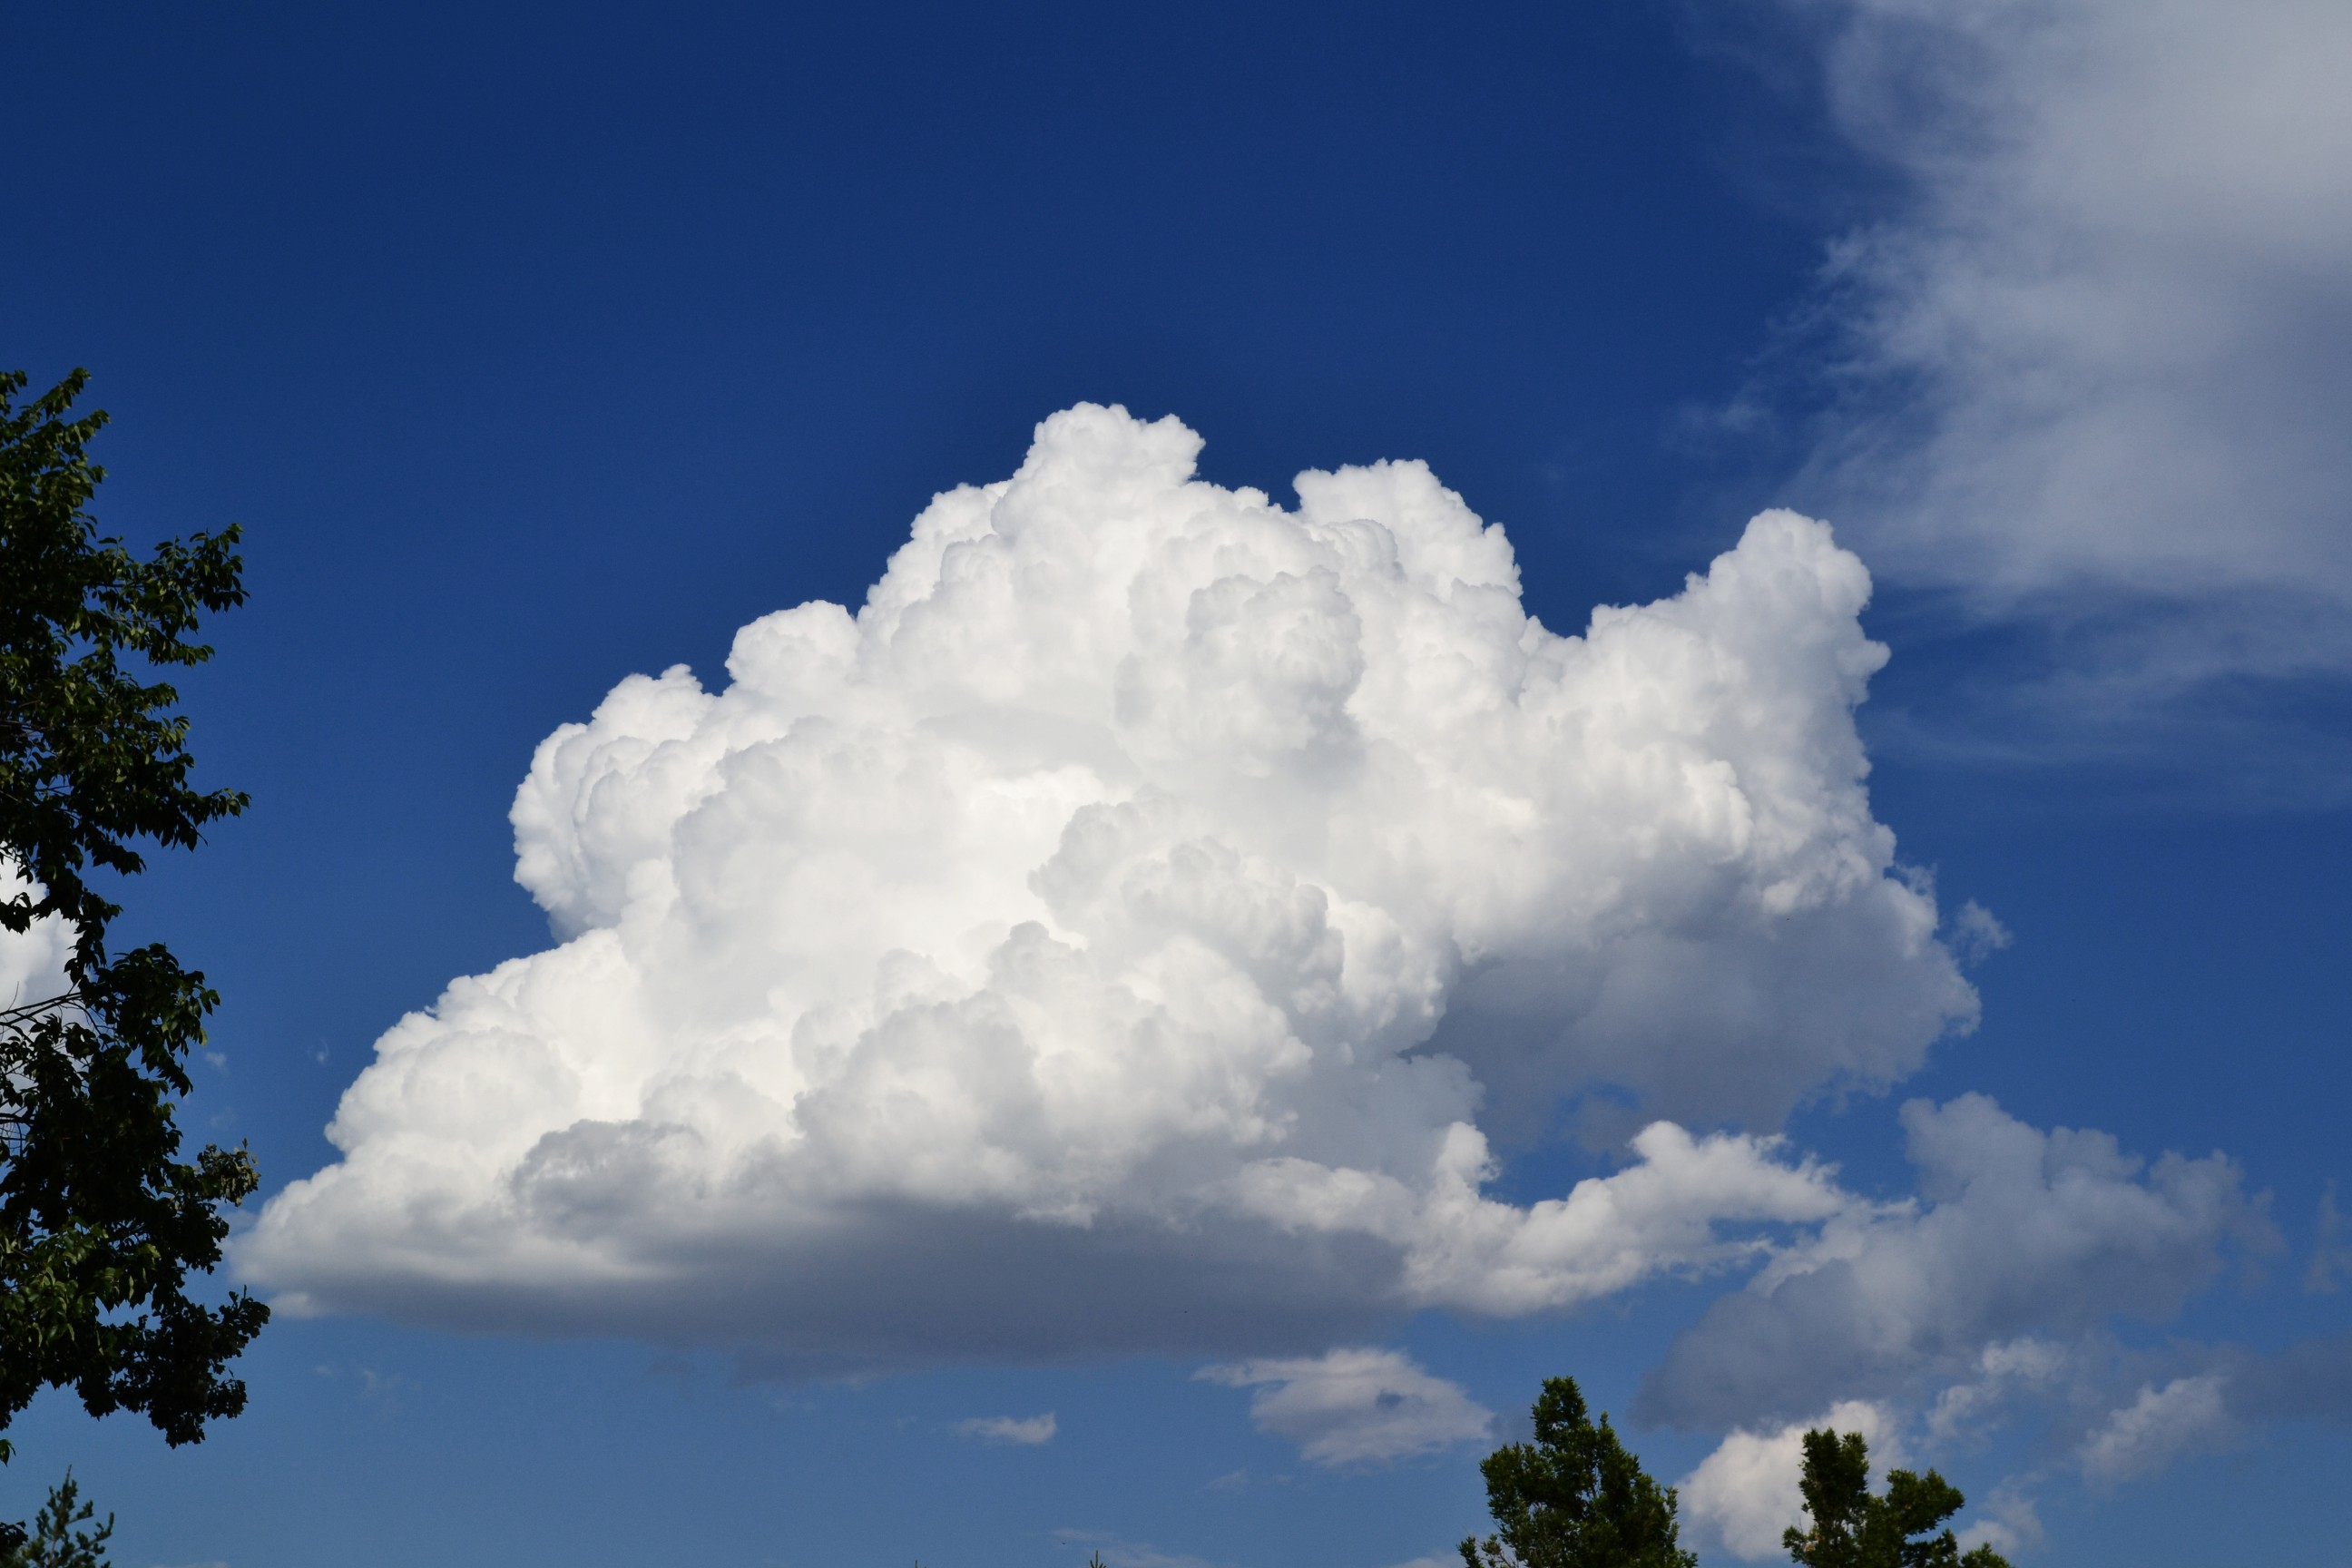
\includegraphics[scale=0.13]{images/single-fluffy-cumulus-cloud-sunny-day-2012-07-26.jpg}
\caption{Single cumulus cloud}
\label{f1}
\end{center}
\end{figure}

Cumulus clouds are a genus-type of low-level cloud that can have noticeable vertical development and clearly defined edges. Cumulo- means "heap" or "pile" in Latin. They are often described as "puffy" or "cotton-like" in appearance, and generally have flat bases. Cumulus clouds, being low-stage clouds, are generally less than 3,300 ft in altitude unless they are the more vertical cumulus congestus form. Cumulus clouds may appear by themselves, in lines, or in clusters.

\subsection{Why does the paper concentrate on rendering cumulus clouds?}
Among the numerous kinds of clouds in the nature environment, cumulus clouds have the most pronounced volumetric feature, making the volumetric rendering more practical. In the final step of the proposed method from the paper, a volume-aware blending is performed. If we use other kind of clouds, such as stratus clouds or cirrus clouds, the volumetric feature can be hardly found, which is not able to be rendered as physically based clouds. This is because we will need a volume to calculate the light occlusion later on.

\section{Existing cloud rendering techniques}
Off-line rendering can be quite accurate about simulating the cloud, but it could take minutes to hours to draw a single frame. We'll be looking into the existing real time rendering methods in the following subsections.

\subsection{Particle Systems (Billboards)}
\begin{figure}[htp]
\begin{center}
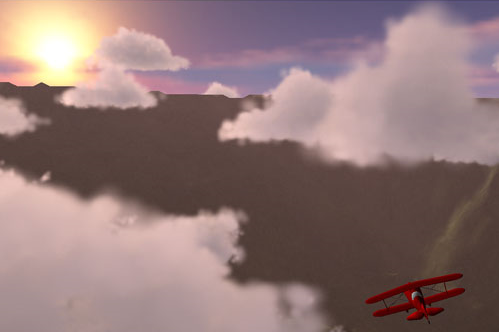
\includegraphics[scale=0.8]{images/billboards.png}
\caption{Billboards Clouds}
\label{f2}
\end{center}
\end{figure}

We simulate and render clouds with billboards, and create shafts of light by rendering concentric semitransparent shells. In this method, the clouds are treated as 3D objects. When the aircraft flies into a cloud, the imposter will be split into 2 pieces, one in front and one behind the aircraft.\\
This method has certain advantages, such as fast, efficient, and the programmer can easily manipulate the shapes and the locations of the billboards. However, as the clouds are represented in a quads facing the camera all the time, the scene will get unrealistic sometimes, for example, when an aircraft flies above the clouds, we will still see the clouds facing the camera as if the we are on the ground. Also the lighting on the billboard is usually precomputed and the clouds are static, which means the clouds will not be able to response to the change of environment.

\subsection{Ray Casting-Based Rendering (Ray Marching)}
\begin{figure}[htp]
\begin{center}

\includegraphics[scale=0.6]{images/raymarching.png}
\caption{Ray Marching Clouds}
\label{f3}
\end{center}
\end{figure}

In this method, we cast rays into the scene and accumulate the volume densities at certain intervals. By applying a volume lighting model on-the-fly or by retrieving the illumination from a pre-computed lighting data structure, the illumination values is then calculated. Also, we represent the cloud density as 3D noise images.\\
This method can result in a fairly realistic output. However, it's not easy for a programmer to control the shape and location of the clouds. Also, in order to do aliasing, the ray marching steps will be tedious. As for the rendering result, the lightings is usually limited to single scattering, which is more or less not so realistic.

\subsection{Rasterization-based Rendering (Volume Rendering)}
\begin{figure}[htp]
\begin{center}
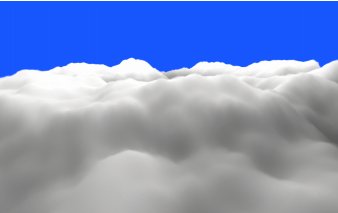
\includegraphics[scale=1.0]{images/volumerendering.png}
\caption{Volume Rendering Clouds}
\label{f4}
\end{center}
\end{figure}

Volume slicing is a straightforward method for rendering regular grids. The slices are usually axis aligned and rendered in front-to-back order (or vice-versa), applying viewing transformations and blending. While volume slicing is not necessarily a rasterization-based method, most algorithms exploit the highly optimized texturing capabilities of the graphics hardware.\\
Splatting became the common method for rendering particle systems. Particles, which are usually specified as independent of rotation, can be rendered by using a textured quad representing the projection of the particle onto a plane, also called splat or footprint. The particles are rendered in back-to-front order, applying blending for semi-transparent volumes. \\
Nowadays, rendering clouds as textured ellipsoids is no more regarded as realistic. The same applies to the surface-bounded clouds of . A triangle mesh is created by surface subdivision of an initial mesh, created by a marching cubes algorithm applied on weather forecast data. The rendering of the semi-transparent mesh, however, is prone to artifacts on the silhouette.